\documentclass[11pt,a4paper,twoside,notitlepage]{article}
%comment out the line above and decomment the one below; the format will change
%\documentclass[conference,a4paper]{IEEEtran}  

%
% Here, you specify the packages you need
%

%You need these 2 packages to write algorithms
\usepackage{algorithmic}
\usepackage{algorithm}
%You need this package to handle figures
\usepackage{graphicx}
%You need this package to write Romanian diacritics properly
\usepackage{combelow}
\usepackage{hyperref}

\usepackage[utf8x]{inputenc} %alternative solution for Romanian diacritics
%This is how you define you own commands/macros
%this is a macro for writing "n choose k" the Romanian style
\newcommand{\mycomb}[2]{{C}_{#1}^{#2}} 
%this is a macro for writing "n choose k" the English style
%\newcommand{\mycomb}[2]{\left( \begin{array}{l}{#2}\\{#1}\\ \end{array} \right)} %this 


%
% The document content starts here
%
\setcounter{tocdepth}{2}
\renewcommand{\contentsname}{Cuprins}
%\setlength{\parindent}{4em}

\begin{document}
% paper title 
\title{Bontida are din nou nevoie de ajutor}

% author names and affiliations
\author{
Student: Gabor George C\u{a}t\u{a}lin\\ %double backslash means linebreak
Grupa: 30239\\
}

%generate paper title
\maketitle 

\newpage

\tableofcontents

%\section*{Cuprins}


\newpage

\section{Analiza cerințelor}

\subsection{Specificare cerinte}
Se cere realizarea unei aplicaiți web pentru prezentarea unui magazin pentru fectivalul Electric Castle. Acesta va avea două tipuri de utilizatori 
\begin{itemize}
	\item administrator;
	\item user normal.
\end{itemize}
fiecare avand diferite privilegii. Nu se cere o implementare pentru un sistem de login.

\subsection{Cerinte functionale}
Aplicația trebuie să pună la dispoziție utilizatorilor următoarele funcționalități:
\begin{itemize}
	\item toate operațile făcute de un utilizator vor fi marcate prin tipul său in URL (ex: pentru admin, URL-ul va avea o formă aseamănatoare cu http://localhost/admin).
	\item pentru user normal:
					\begin{itemize}
						\item	vizualizare listă cu produsele disponibile;
						\item 	vizualizarea ierarhie de categorii a produselor;
						\item 	filtrarea produselor prin selectarea unei categorii.
					\end{itemize}
	\item pentru administrator:
					\begin{itemize}
						\item	toate operațile unui user normal;
						\item	adăugare produse într-o categorie;
						\item	stergere produse;
						\item	adăugarea de subcategorii categoriilor existente;
						\item 	ștergerea de subcategorii.
					\end{itemize}
\end{itemize}

\subsection{Cerinte non-functionale}
Urmatoarele cerinte trebuie respectate:
\begin{itemize}
	\item 	utilizarea unui framework ce implementează patternul MVC (Spring Boot);
	\item	utilizarea unui frameword Object-Relational Mapping (JPA);
	\item 	datele stocate într-o bază de date (MySql);
	\item 	utilizaera pattern-ului Composite;
	\item	timpul de raspuns al sistemului pentru orice operatie trebuie sa fine mai mic de 2 secunde;
	\item	arhitectura sistemului trebuie sa permina adaugarea de noi operatii sau modificarea celor curente;
\end{itemize}

\section{Use Case Model}

Use case: Adăugarea unui produs; \\
Level: User-goal; \\
Actor princital: Admin; \\
Scenariu de succes: După analizarea ierarhiei, utilizatorul introduce numele, prețul și id-ul (categoriei în care se dorește adăugarea) și se apasă butonul ADD. Produsul va apărea apoi în lista de produse; \\
Extensii: Operatia poate eșua dacă:
\begin{itemize}
	\item id-ul introdus nu corespunde nici unei categorii;
	\item în cămpul pentru preț se introduc date eronate;	
	\item intervine o problemă în baza de date.
\end{itemize}
\newpage
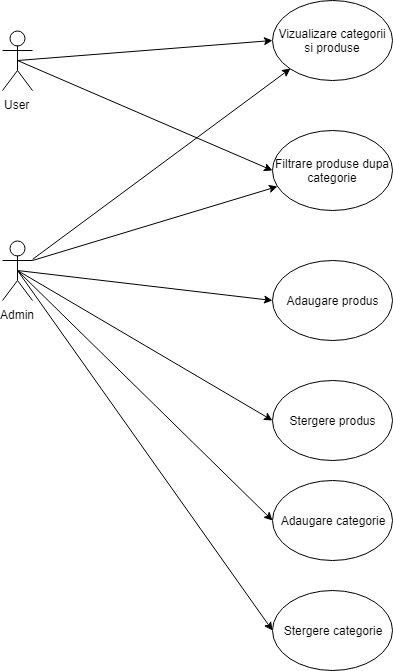
\includegraphics[height=.5\textheight]{useCases}


\section{Design-ul arhitectural al sistemului}

\subsection{Descrierea modelului arhitectural}
Este utilizat pattern-ul arhitectural MVC.\\
Aplicatia este compusa din trei nivele: 
\begin{itemize}
	\item View - contine interfata cu utilizatorul, în cazul nostru este web; 
	\item Controller - leaga Modelul de View și procesează toate cererile;
	\item Model - oferă acces structurat la date. Acesta este împărtit în alte trei părți:
																	\begin{itemize}
																		\item Entities - structurile de date;
																		\item Repositories - accesul la baza de date;
																		\item Services - combină Entities și Repositories pentru a returna date structurate.
																	\end{itemize}
\end{itemize}

\subsection{Diagrame}

Urmatoarea diagrama prezinta structura pachetelor din sistem :
\newpage
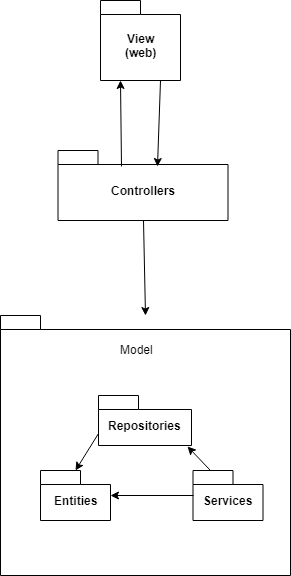
\includegraphics[height=.4\textheight, width=.4\textwidth]{packages} \\
\\
Diagrama de componente: \\
\\
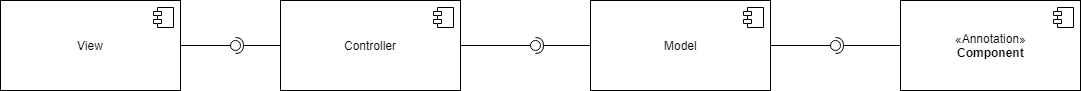
\includegraphics[width=.6\textheight]{components} \\
\\
Diagrama de deployment: \\
\\
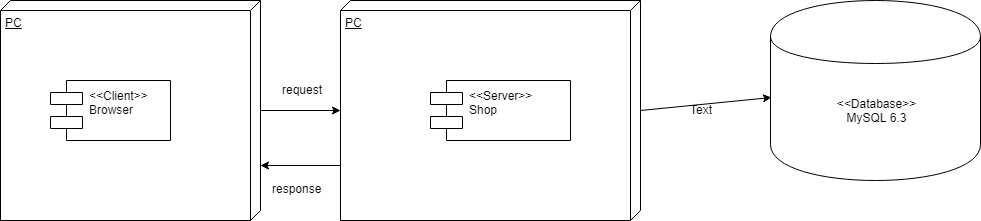
\includegraphics[width=.6\textheight]{deployment} \\


\section{Diagrame de secventa UML}
Consideram scenariul în care administratorul dorește să adauge un produs: \\
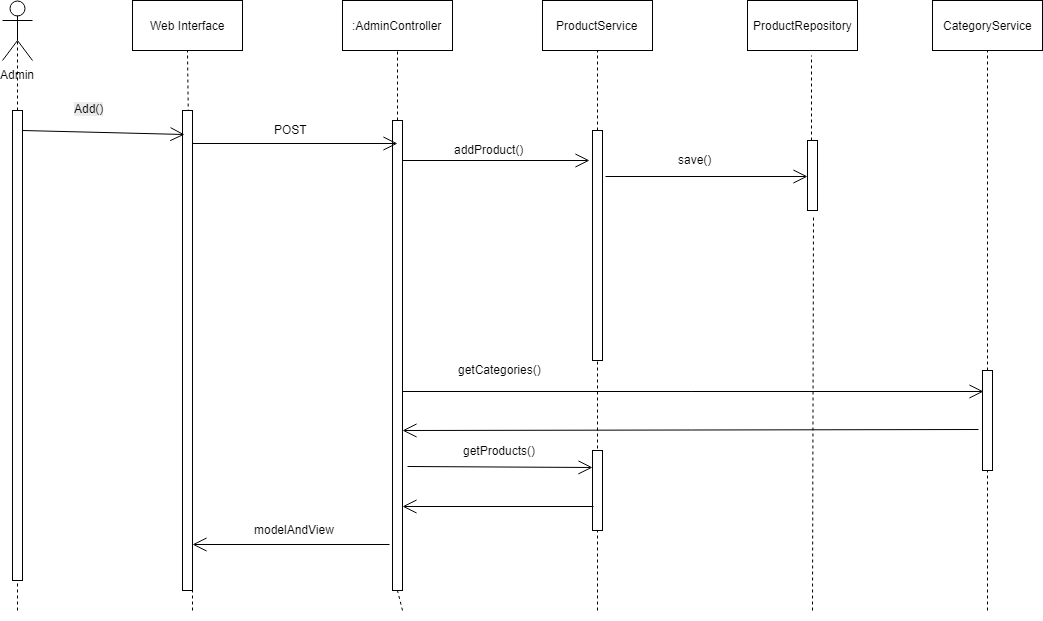
\includegraphics[width=.6\textheight]{secventa}


\section{Design-ul claselor}

\subsection{Descriere design pattern-uri utilizate}

Au fost utilizate urmatoarele:
\begin{itemize}
	\item Composite - Clasele Product și Category formează o ierarhie, o instanță a clasei Category conține o listă de instanțe a clasei Product;
	\item Repository - ProductRepository și CategoryRepository se ocupă de accesul la baza de date;
\end{itemize}

\newpage
\subsection{Diagrama de clase}
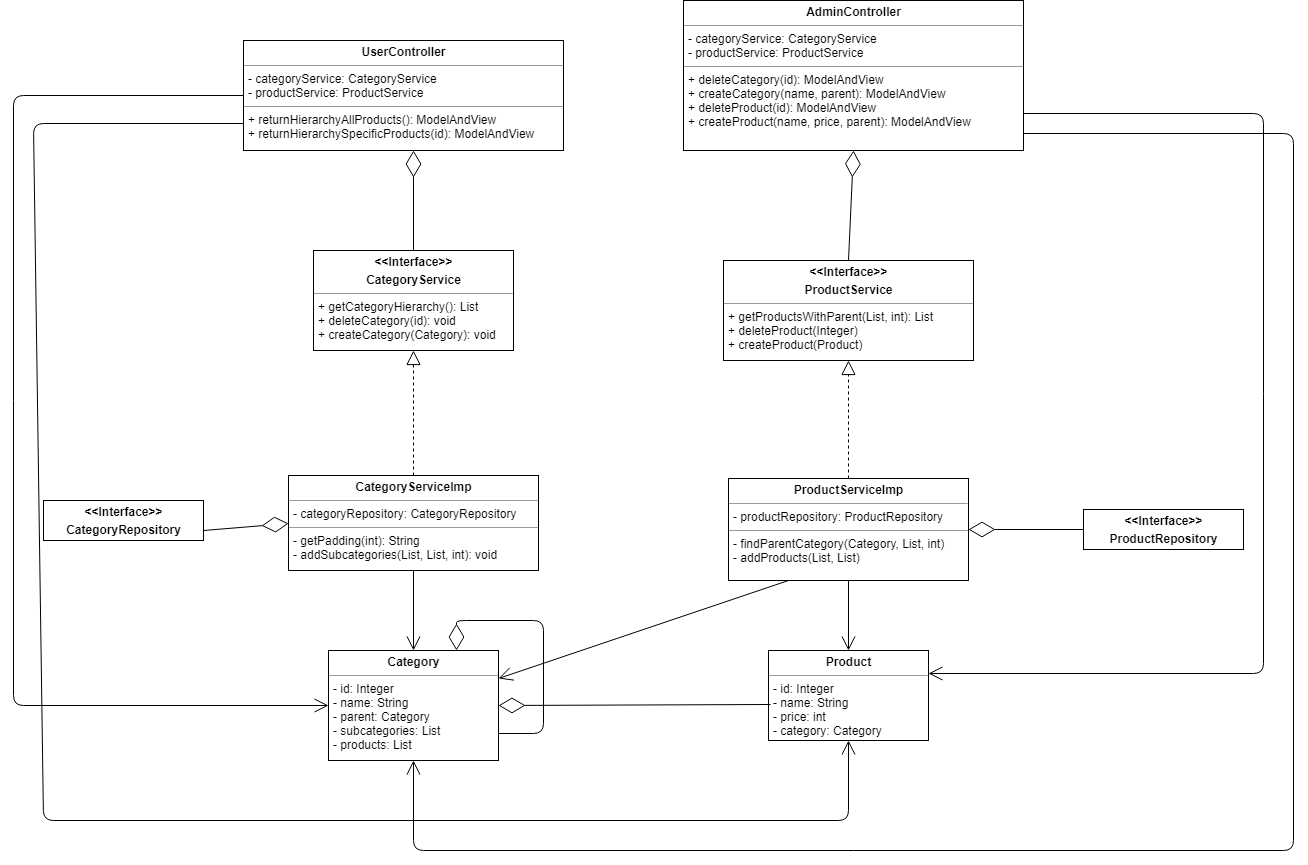
\includegraphics[height=.5\textheight, width=1\textwidth]{class}
\newpage

\section{Model de date}

Baza de date in care sunt stocate informatiile este urmatoare: \\
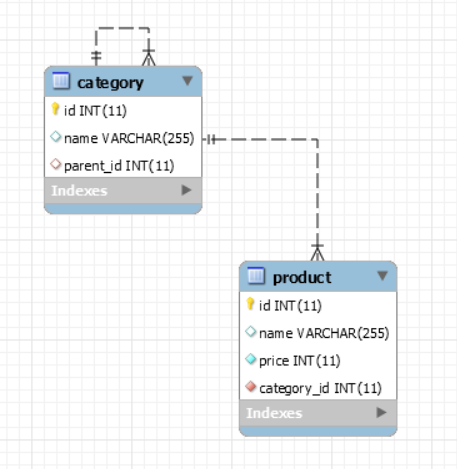
\includegraphics[height=.5\textheight, width=.8\textwidth]{database} \\
Dupa cum se poate, vedea exista două tabele:
\begin{itemize}
	\item Product - atributul category\_id face legătura unui produc cu o categorie;
	\item Category - atributul parent\_id leaga o categorie de o subcategorie.
\end{itemize}


\section{Testarea sistemului}

S-a folosit o strategie de testare incrementală, funcționalitățile au fost verificate pe măsură ce au fost adăugate in sistem. Astfel, principalele metode de testare au fost data-flow (au fost date anumite intrări si s-a observat raspunsul sistemului), white-box (codul a fost disponibil).

\section{Bibliografie}

Pentru utilizare Spring Boot și JPA:
\begin{itemize}
	\item \url{https://www.youtube.com/watch?v=msXL2oDexqw&list=PLqq-6Pq4lTTbx8p2oCgcAQGQyqN8XeA1x}  \\
\end{itemize}
Pentru anumite erori și html:
\begin{itemize}
	\item \url{https://stackoverflow.com/}
	\item \url{https://www.youtube.com/}	
\end{itemize}

\end{document}
